\todo[inline]{\textbf{TODO:} Write section introduction.}

\subsection{Sizing}
\todo[inline]{\textbf{TODO:} Short introduction.}

\subsubsection{Solar Array}
Equation \ref{eq:SA_slope_energy} is rearranged in into an expression of the solar cell coverage area $A$, shown in Equation \ref{eq:solar_cell_coverage_area}:

\begin{equation}
  \label{eq:solar_cell_coverage_area}
  A = \frac{E}{\eta \cdot H_{\beta} \cdot PR}
\end{equation}

where $E$ becomes the energy required by the rover on that Sol and $H_{h}$ the worst-case available daily insolation, henceforth $E_{req}^{worst}$ and $H_{\beta}^{worst}$ respectively. $H_{\beta}^{worst}$ is used instead of $H_{h}^{worst}$ in order to take advantage of the rover's active suspension system to generate the most available worst case daily insolation. The values for these varibles are taken from assumptions and previously calculated energies and daily insolations:

\begin{enumerate}[label=\textbf{\textcolor{BulletBlue}{(\alph*)}}]
    \item From Table \ref{tab:worst-case-traverse-sol-power-budget}, $E_{req}^{worst}$ is \SI{775}{\watt\hour} at Iani Chaos and \SI{750}{\watt\hour} at Ismenius Cavus.
    \item From Tables \ref{tab:insolation-iani-chaos-clear-and-dusty-days} and \ref{tab:insolation-ismenius-cavus-clear-and-dusty-days}, $H_{\beta}^{worst}$ for $\tau=1$ is \SI{2479}{Wh.m^{-2}} at Iani Chaos and \SI{1345}{Wh.m^{-2}} at Ismenius Cavus.
    \item From \ref{itm:ass:red_shifts}, \ref{itm:ass:dust_deposition_saturation}, and \ref{itm:ass:protruding_shadowing}, \ac{PR} at \ac{EOL} is $PR_{EOL} = 1 - (0.03 + 0.3 + 0.05) = 0.62$.
    \item From \ref{itm:ass:solar_cell_efficiency}, $\eta_{EOL} = 0.22$.
\end{enumerate}


The required solar cell coverage area at Iani Chaos was thus determined:
\begin{align}
  \label{calc:solar_cell_area_iani_chaos}
  A_{iani} &= \frac{E_{req}^{worst}}{\eta_{EOL} \cdot H_{\beta}^{worst} \cdot PR_{EOL}}\\
           &= \frac{775}{0.22 \cdot 2479 \cdot 0.62}\\
           &= \SI{2.29}{m^{2}}
\end{align}

and at Ismenius Cavus:
\begin{align}
  \label{calc:solar_cell_area_ismenius_cavus}
  A_{ismenius} &= \frac{E_{req}^{worst}}{\eta_{EOL} \cdot H_{\beta}^{worst} \cdot PR_{EOL}}\\
               &= \frac{750}{0.22 \cdot 1345 \cdot 0.62}\\
               &= \SI{4.09}{m^{2}}
\end{align}

At Iani Chaos, from \ref{itm:ass:packing_efficiency} the resulting \ac{SA} area was \SI{2.7}{m^{2}} and from \ref{itm:ass:sa_surface_density} its mass was 9.95 \si{\kilo\gram}. Taking advantage of \ac{SA} inclination capabilities with $\beta_{best} = \SI{10}{\degree}$ resulted in \ac{SA} sizing decrease of \SI{3.9}{\percent} when compared with a horizontal surface configuration. For $\tau = 1$ during global dust storm season and $\tau = 0.4$ for the remainder of the year, the total maximum flat traverse distance achievable over the course of one \ac{MY} was increased by \SI{8.79}{\percent} from \SI{59.13}{\kilo\meter} to \SI{64.33}{\kilo\meter}.

At Ismenius Cavus, the resulting \ac{SA} area and mass were \SI{4.8}{m^{2}} at 17.8 \si{\kilo\gram}. The \ac{SA} area was decreased by \SI{4.6}{\percent}. The total maximum achievable flat traverse distance achievable during one \ac{MY} was increased by \SI{1.39}{\percent} from \SI{67.4}{\kilo\meter} to \SI{68.34}{\kilo\meter}.

The traverse distance gains attributed to \ac{SA} inclination capabilities did not seem to justify adopting the complexities of an active suspension system for the purpose of increasing traverse distance via solar tracking. This was particularly true at Ismenius Cavus. The savings in \ac{SA} surface area and mass also left much to be desired. The size problem of the resulting \ac{SA} areas are illustrated in Figure \ref{fig:sa-area-initial-sizes}.

\clearpage
\begin{figure}[h]
  \centering
  \hypersetup{linkcolor=captionTextColor}
  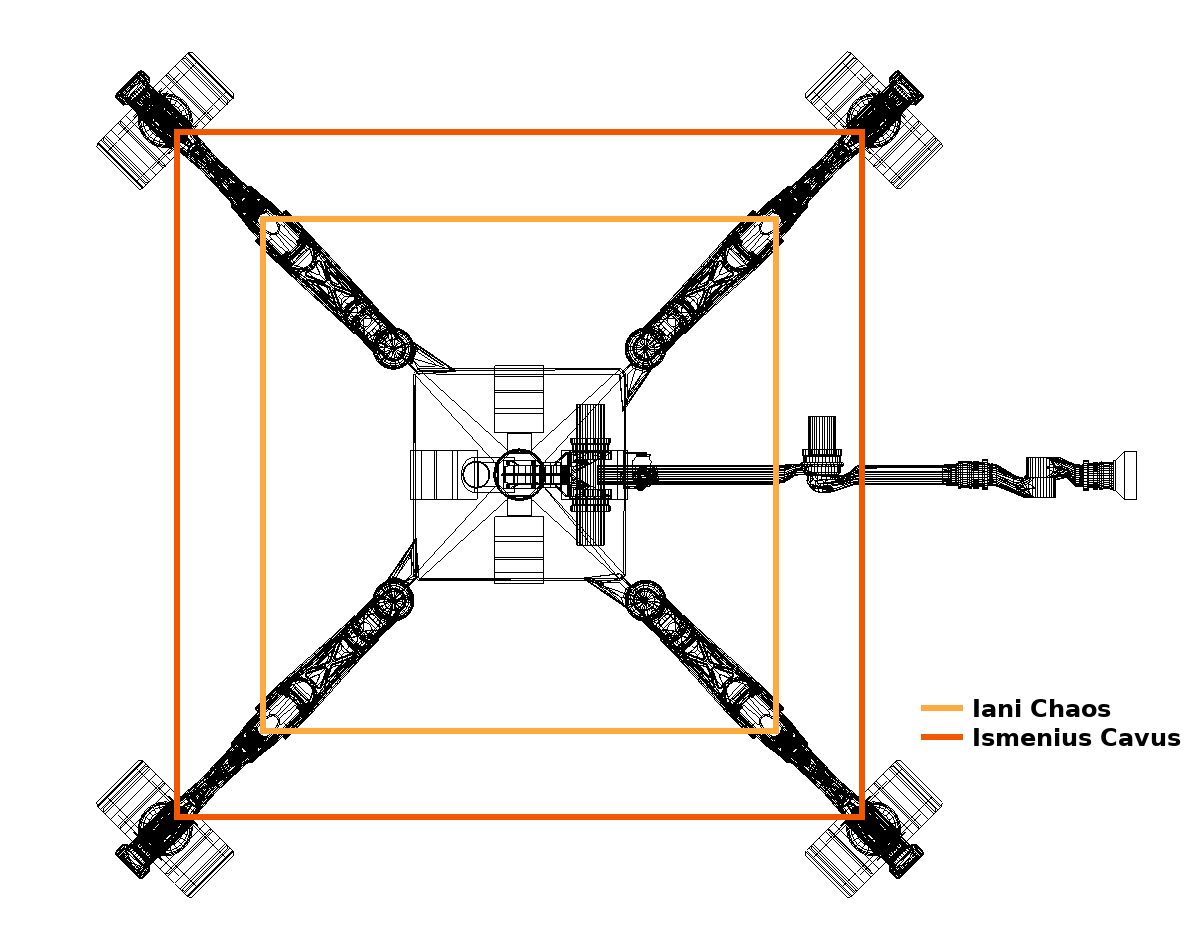
\includegraphics[width=0.8\linewidth]{sections/design/solar-array/images/sa-area-initial-sizes.png}\\
  \caption[Size comparison between SherpaTT and initial SA areas for Iani Chaos and Ismenius Cavus]
          {Size comparison between SherpaTT and initial \ac{SA} areas for Iani Chaos and Ismenius Cavus. The outlined square areas are equivalent to \ac{SA} areas of \SI{2.7}{m^{2}} for Iani Chaos and \SI{4.8}{m^{2}} for Ismenius Cavus.}
  \label{fig:sa-area-initial-sizes}
\end{figure}

To explain the lack of significant gain with $\beta_{best}$, the generated \ac{SA} energy and maximum traverse durations are plotted in Figures \ref{fig:plot:iani-chaos-generated-energy-and-max-traverse-durations} for Iani Chaos and Figure \ref{fig:plot:ismenius-cavus-generated-energy-and-max-traverse-durations} for Ismenius Cavus.

The \ref{itm:con:daylight_traverse} constraint imposed an upper limit to the maximum traverse durations. This ceiling corresponded to the daylight time that was available for traversing. At Iani Chaos, this resulted in the \ac{SA} generating excess propulsion energy which could not be used. For the scenario plotted in Figure \ref{fig:plot:sub:ismenius-cavus-max-traverse-durations}, this occured before and after the global storm season where both horizontal and $\beta_{best}$ inclined \ac{SA} surfaces generated excess energy which annulled any gains associated with solar tracking. This would have also have been the case during the global storm season for clear days with $\tau = 0.4$.

At Ismenius Cavus, the excess energy problem was further pronounced than in Iani Chaos. As seen in the scenario plotted in Figure \ref{fig:plot:sub:iani-chaos-max-traverse-durations}, an inclined \ac{SA} surface was only relevant during the global dust storm season with a dusty atmosphere of $\tau = 1$. This negligeable advantage resulted in the limited \SI{1.39}{\percent} traverse distance gain with $\beta_{best}$ that was noted earlier.

The \ac{SA} sizing approach using Equations \ref{calc:solar_cell_area_iani_chaos} and \ref{calc:solar_cell_area_ismenius_cavus} had to be re-evaluated towards a solution that resulted in significant gains with $\beta_{best}$, bot in terms of \ac{SA} area reduction and in attainable traverse distances when compared to hose obtained from a horizontal \ac{SA} surface.


\begin{figure}[h]
\captionsetup[subfigure]{justification=centering}
\vspace{-2ex}
	\centering
    %% setup sizes
    \setlength{\subfigureWidth}{0.50\textwidth}
    \setlength{\graphicsHeight}{80mm}
    %% kill hyper-link highlighting
    \hypersetup{hidelinks=true}%
    %% the figures
    \begin{subfigure}[t]{\subfigureWidth}
        \centering
        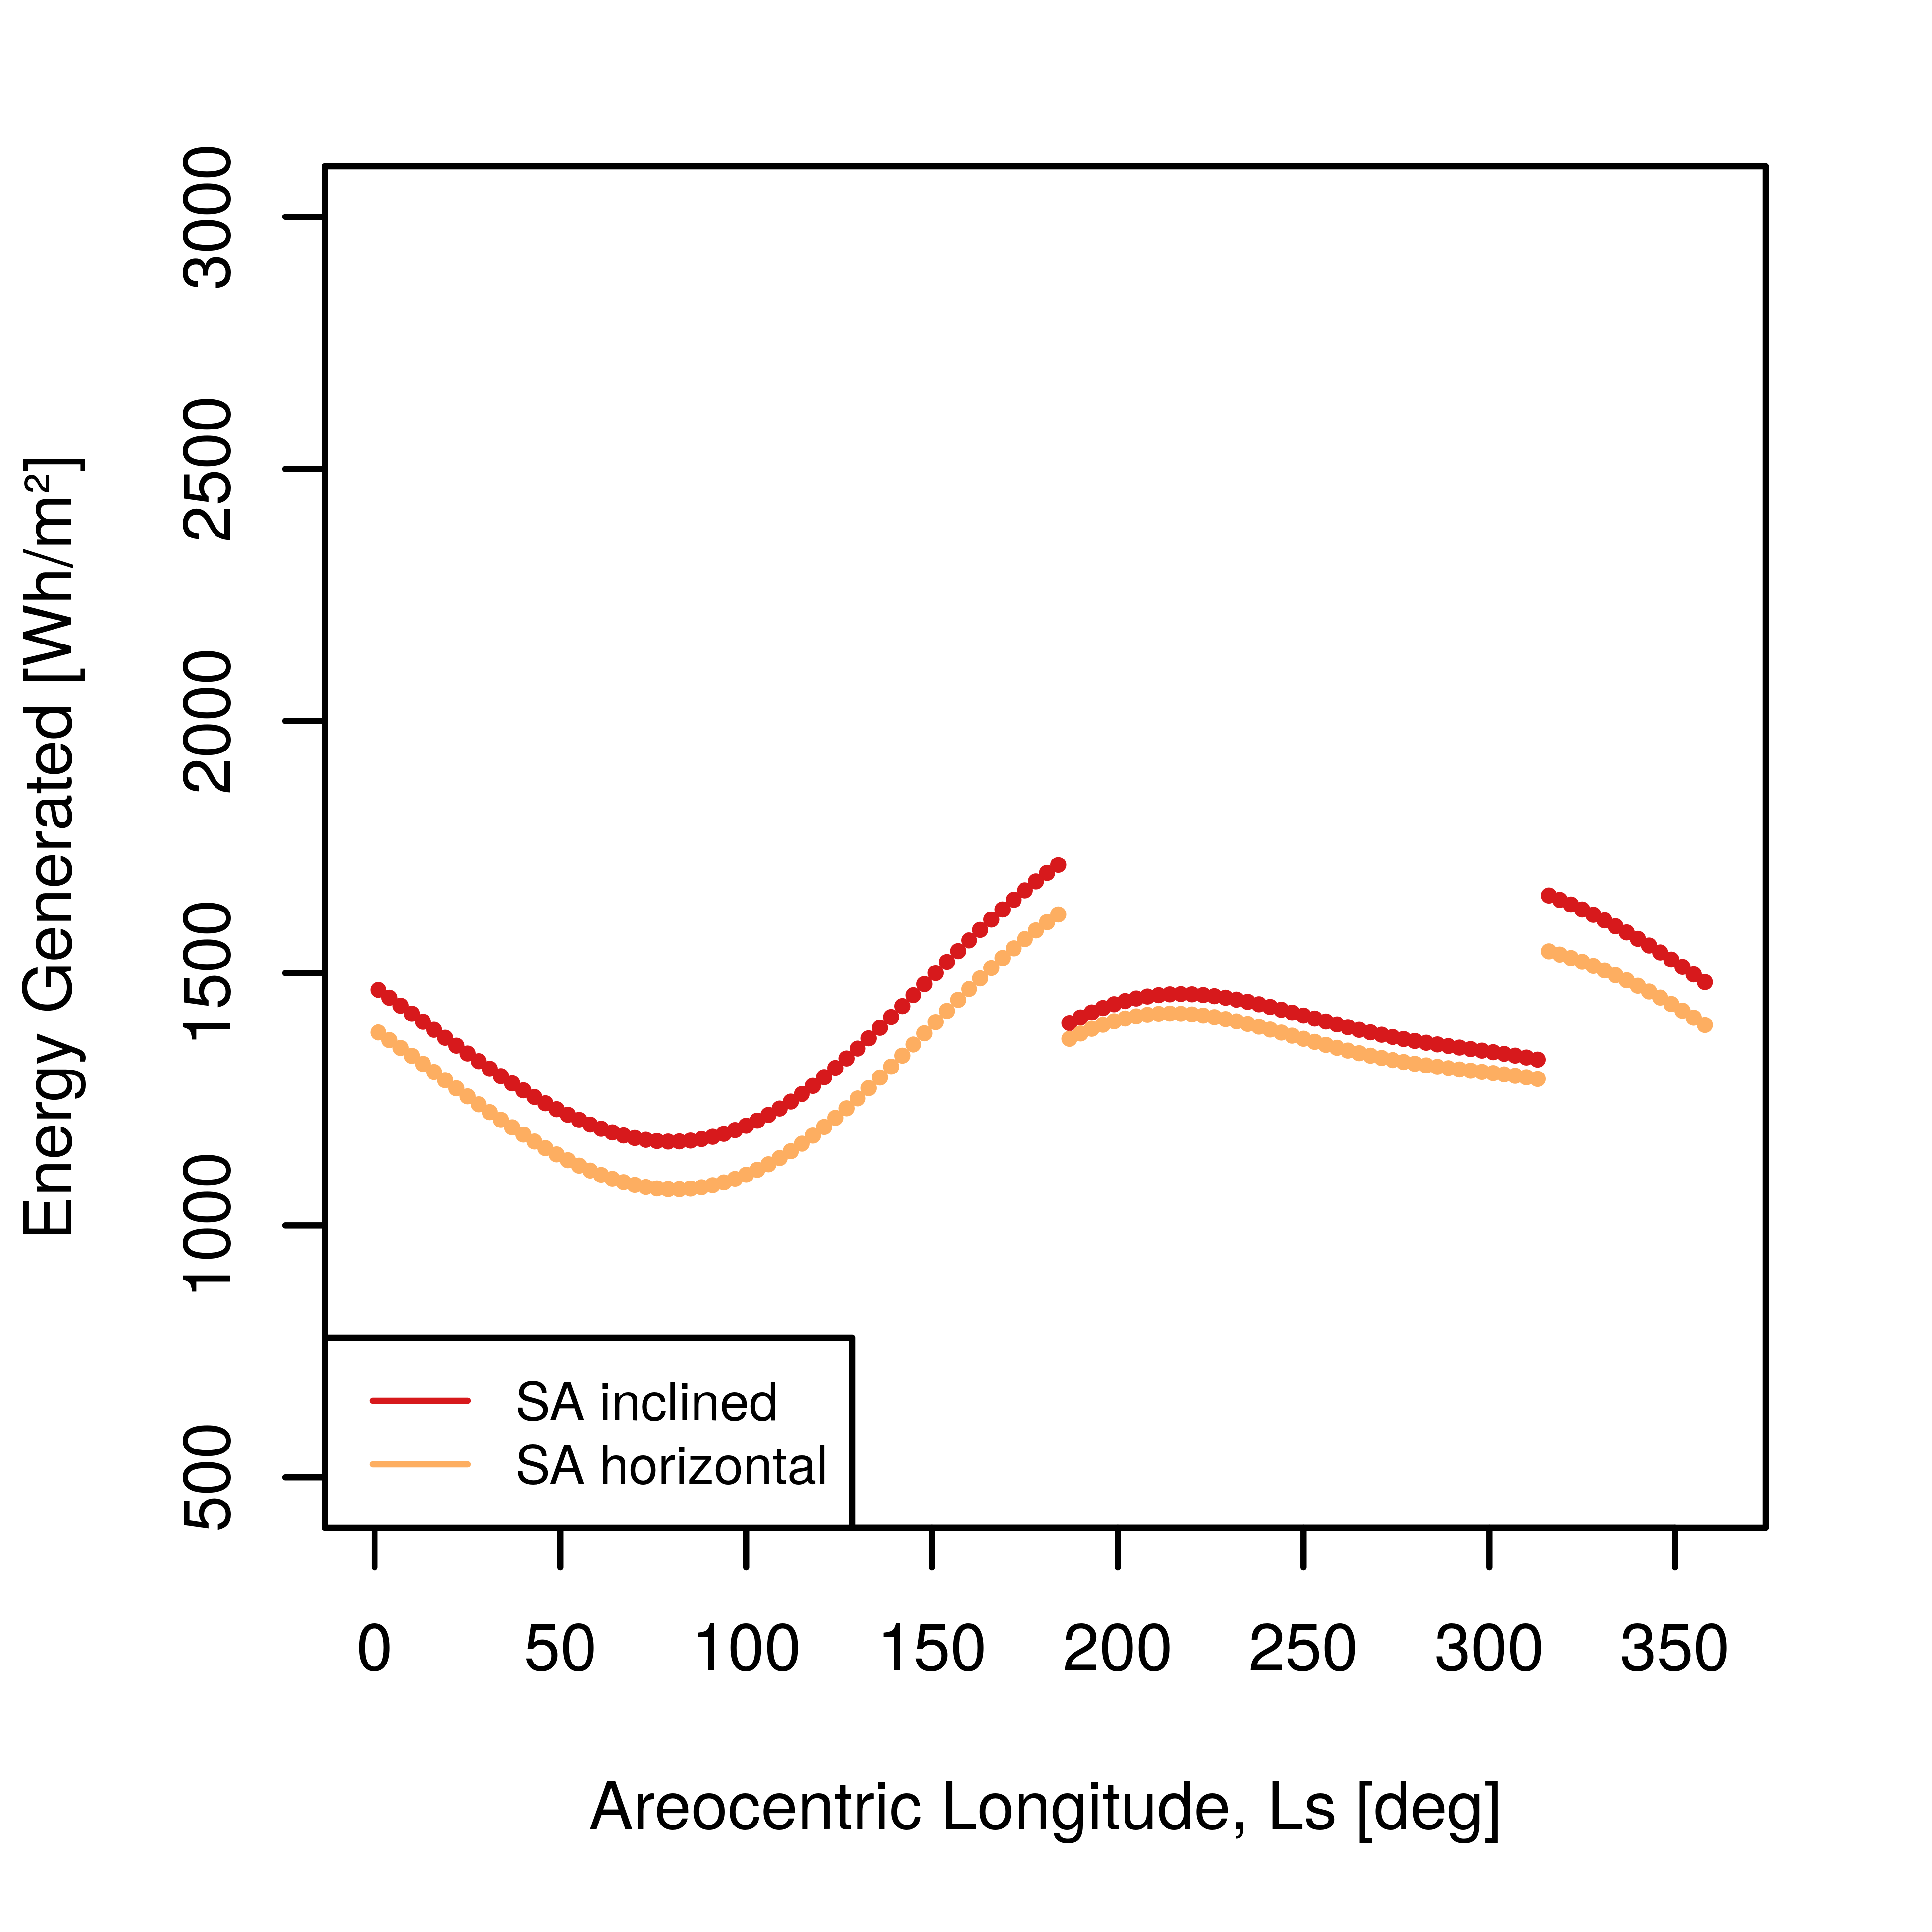
\includegraphics[height=\graphicsHeight]{sections/design/solar-array/plots/ianichaos-daily-generated-energy.png}
        \subcaption{Generated Energy}
        \label{fig:plot:sub:iani-chaos-generated-energy}
    \end{subfigure}\hfill
    \begin{subfigure}[t]{\subfigureWidth}
        \centering
        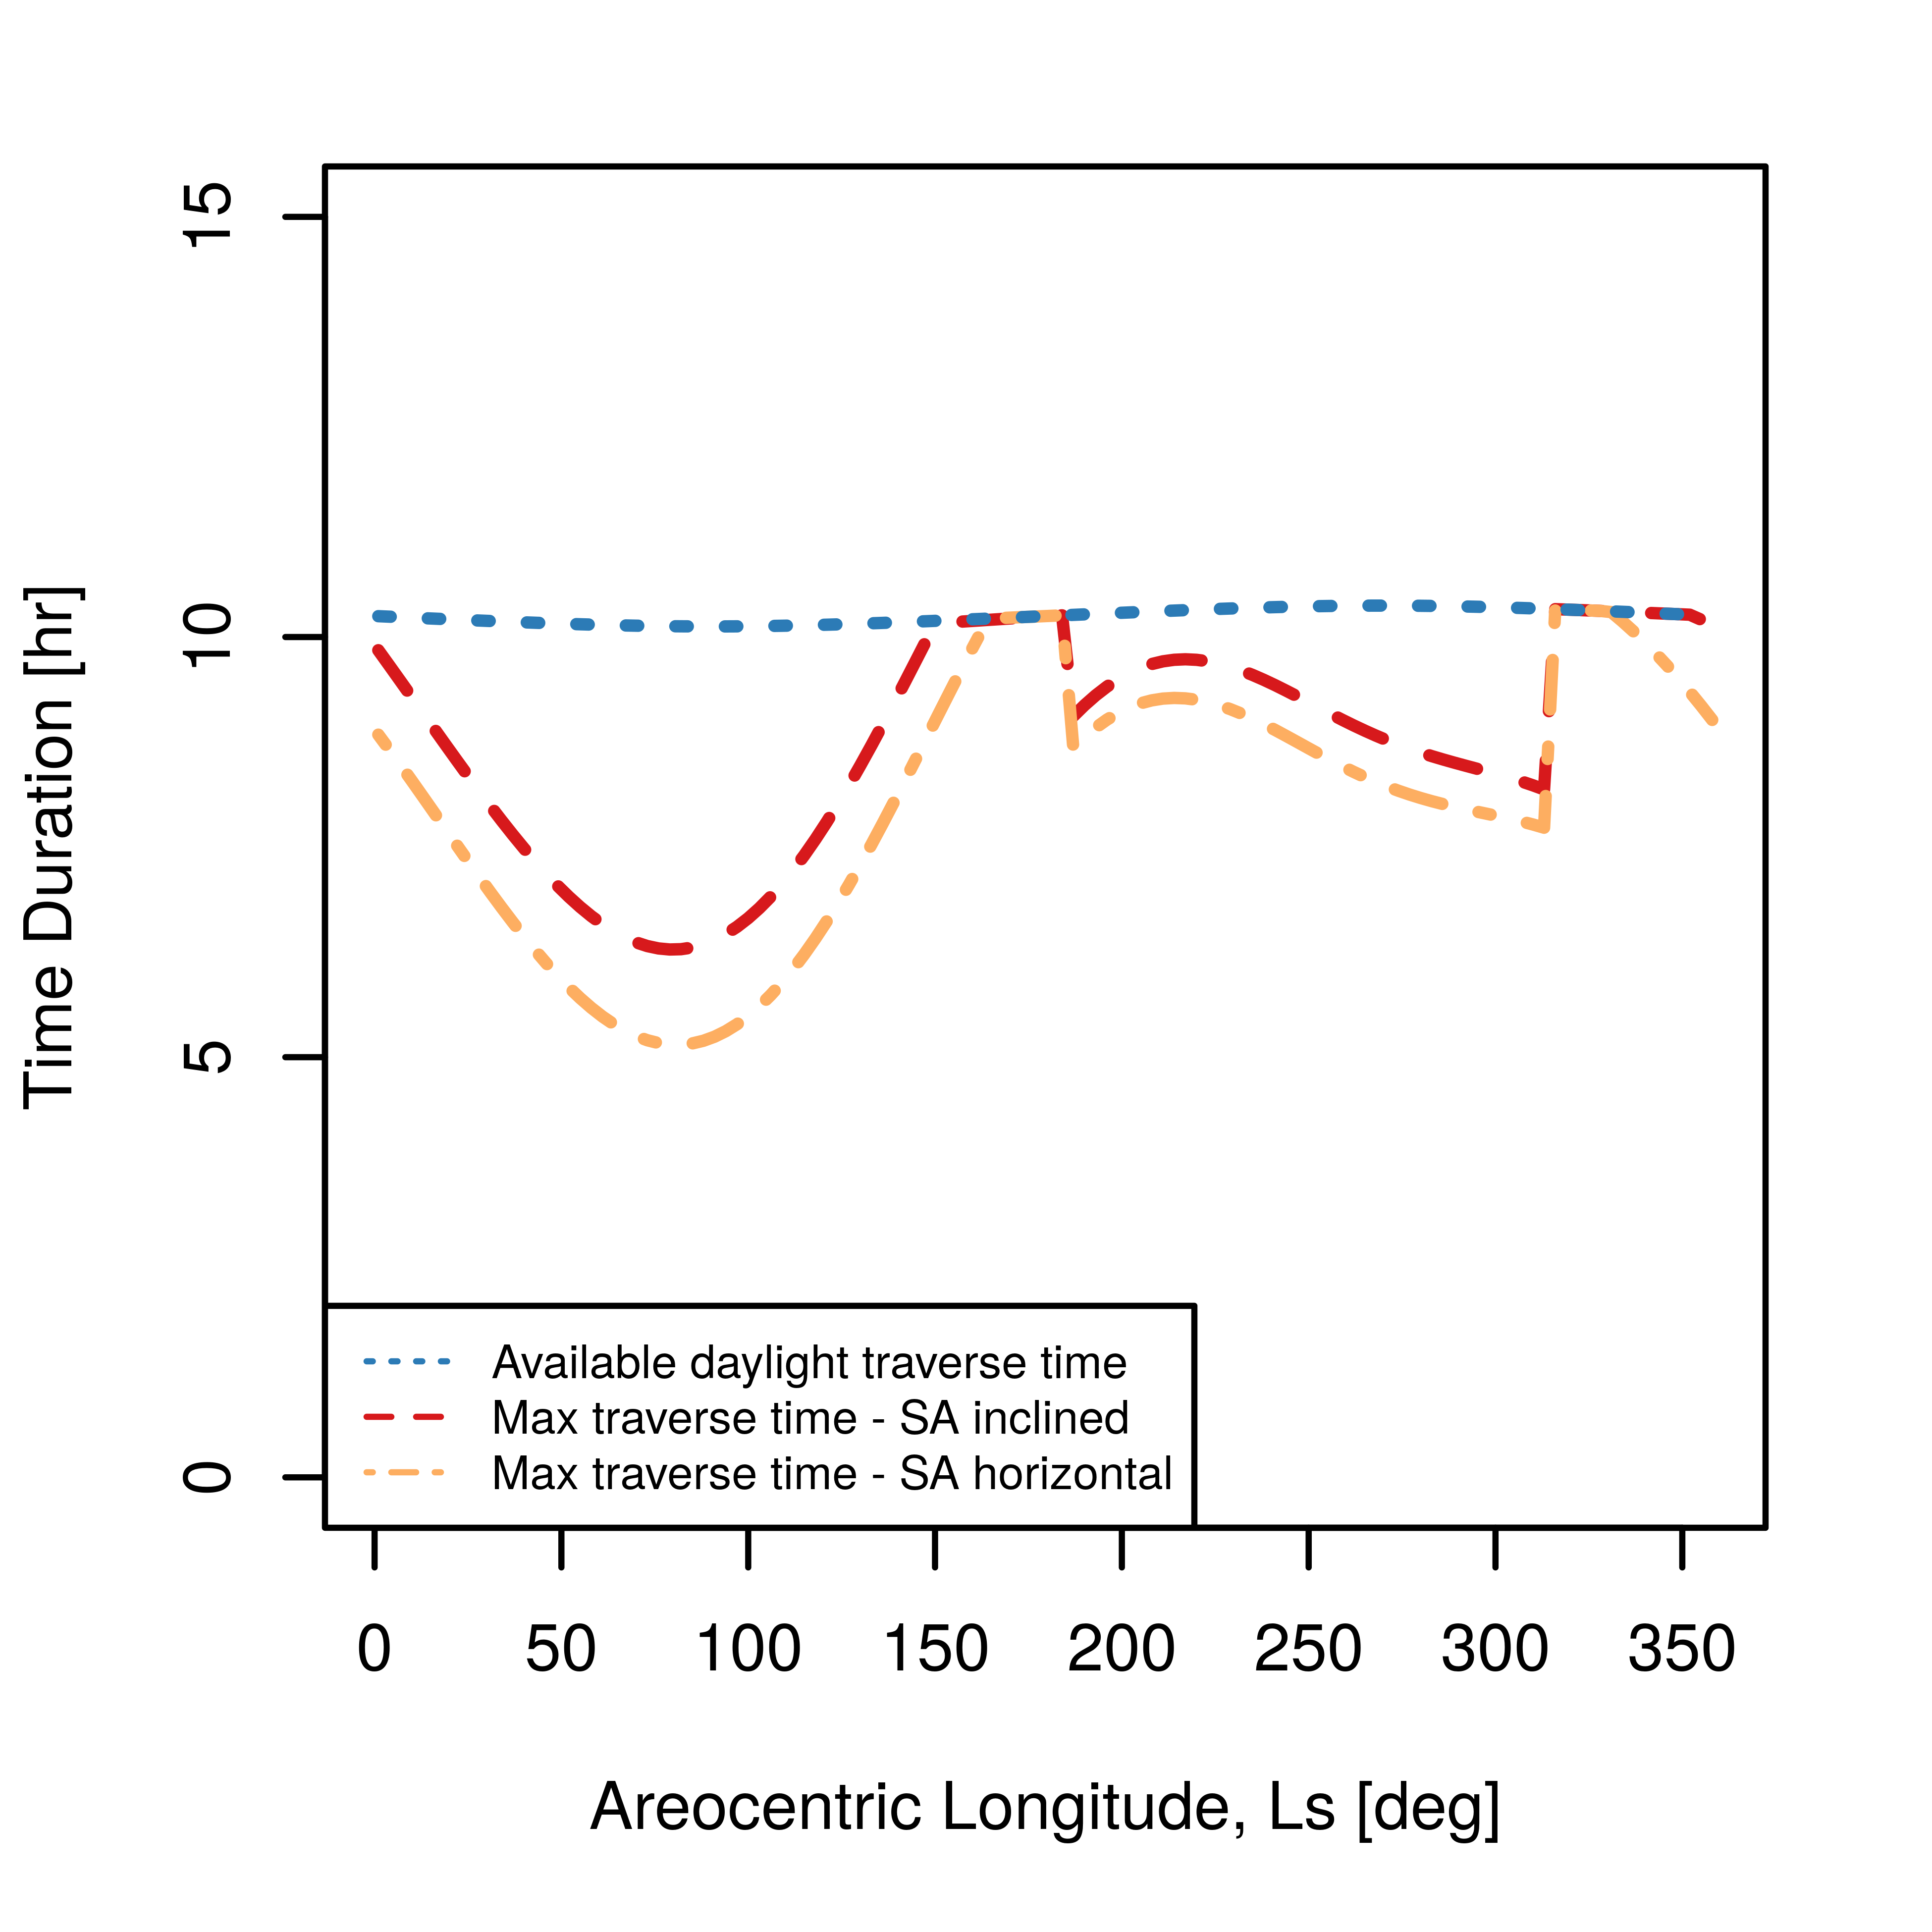
\includegraphics[height=\graphicsHeight]{sections/design/solar-array/plots/ianichaos-75w-max-traverse-durations.png}
  		\subcaption{Maximum Traverse Durations}
		\label{fig:plot:sub:iani-chaos-max-traverse-durations}
	\end{subfigure}\\[0.8ex]
    \caption[Generated energy and maxium achievable flat terrain traverse durations at Iani Chaos]
            {Generated energy and maxium achievable flat terrain traverse duration at Iani Chaos. Optical depth  $\tau = 1$ was used for global dust storm season ($\SI{185}{\degree} \leq L_{s} \leq \SI{315}{\degree}$) and $\tau = 0.4$ for the remainder of the year. The \textit{available daylight traverse time} corresponds to the amount of daylight hours left in a \textit{Traverse Sol} after subtracting the time taken by non-Traverse modes: \textit{Idle - Day}, \textit{\ac{DTE} Communication}, \textit{Science Stop - Short}, and \textit{Optimal Pose}. The maximum traverse durations for \ac{SA} horizontal do not consider the \textit{Optimal Pose} mode.}
    \label{fig:plot:iani-chaos-generated-energy-and-max-traverse-durations}
\vspace{-2ex}
\end{figure}

\begin{figure}[h]
\captionsetup[subfigure]{justification=centering}
\vspace{-2ex}
	\centering
    %% setup sizes
    \setlength{\subfigureWidth}{0.50\textwidth}
    \setlength{\graphicsHeight}{80mm}
    %% kill hyper-link highlighting
    \hypersetup{hidelinks=true}%
    %% the figures
    \begin{subfigure}[t]{\subfigureWidth}
        \centering
        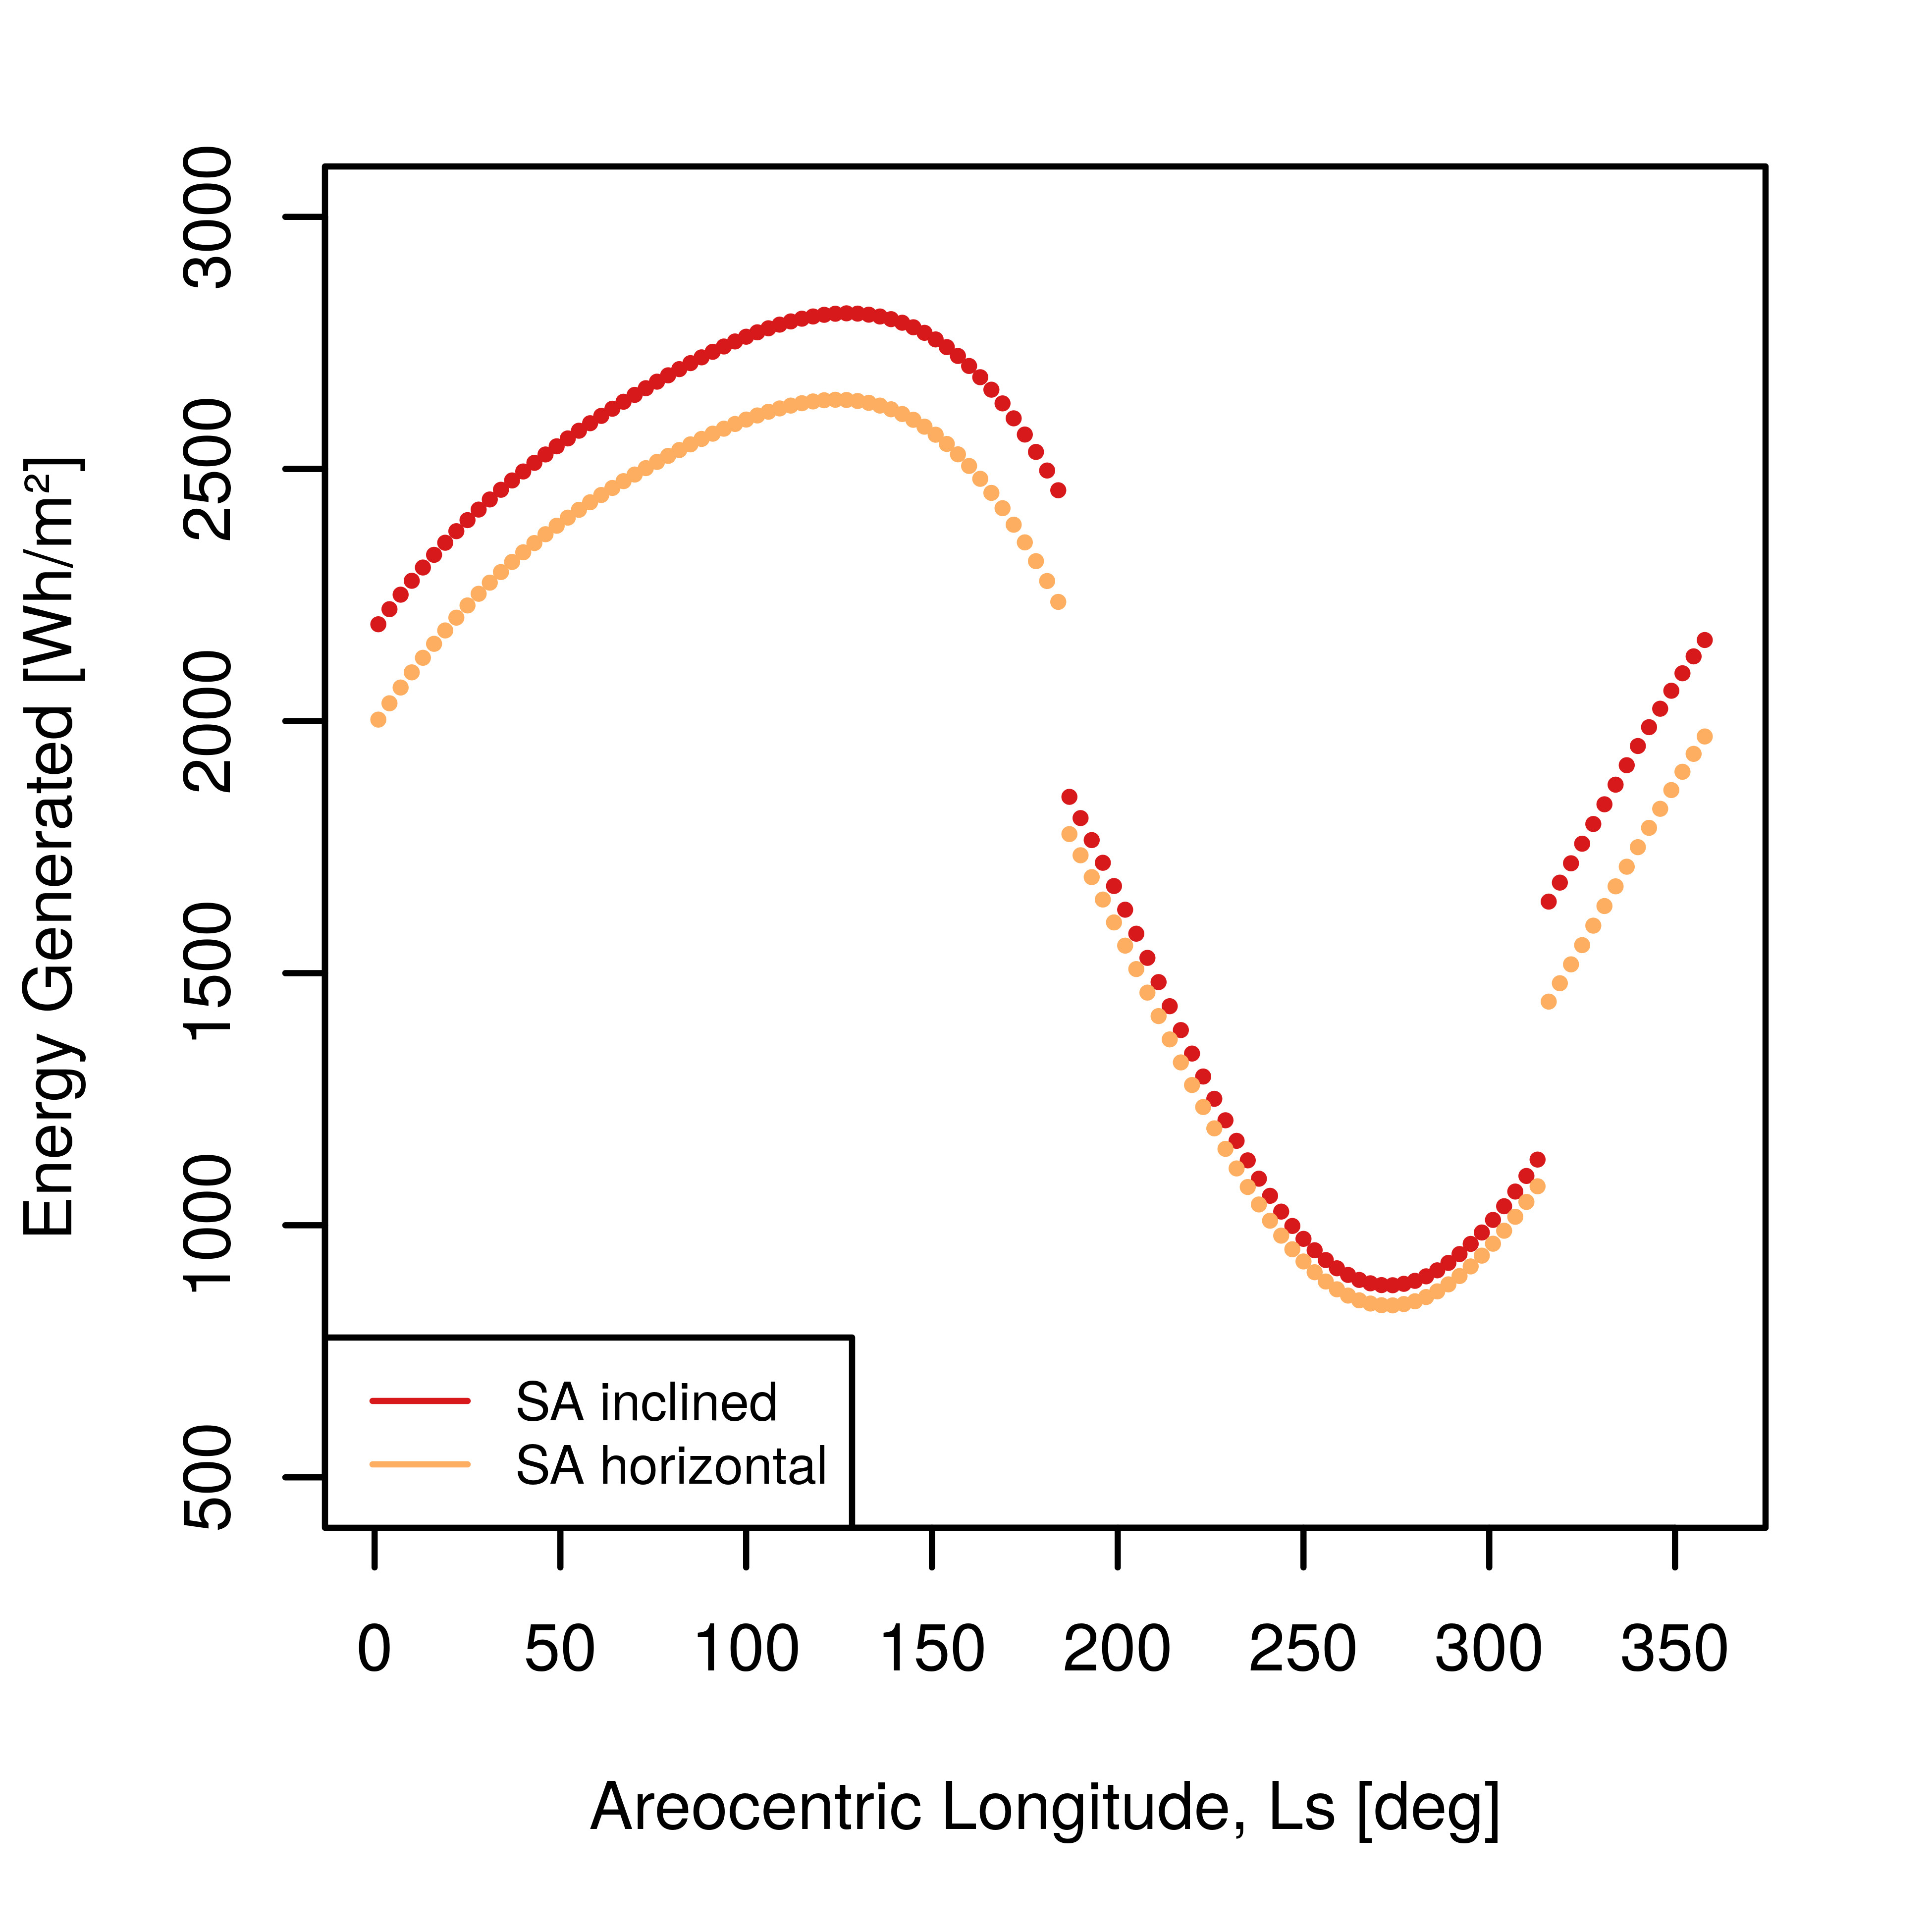
\includegraphics[height=\graphicsHeight]{sections/design/solar-array/plots/ismeniuscavus-daily-generated-energy.png}
        \subcaption{Generated Energy}
        \label{fig:plot:sub:ismenius-cavus-generated-energy}
    \end{subfigure}\hfill
    \begin{subfigure}[t]{\subfigureWidth}
        \centering
        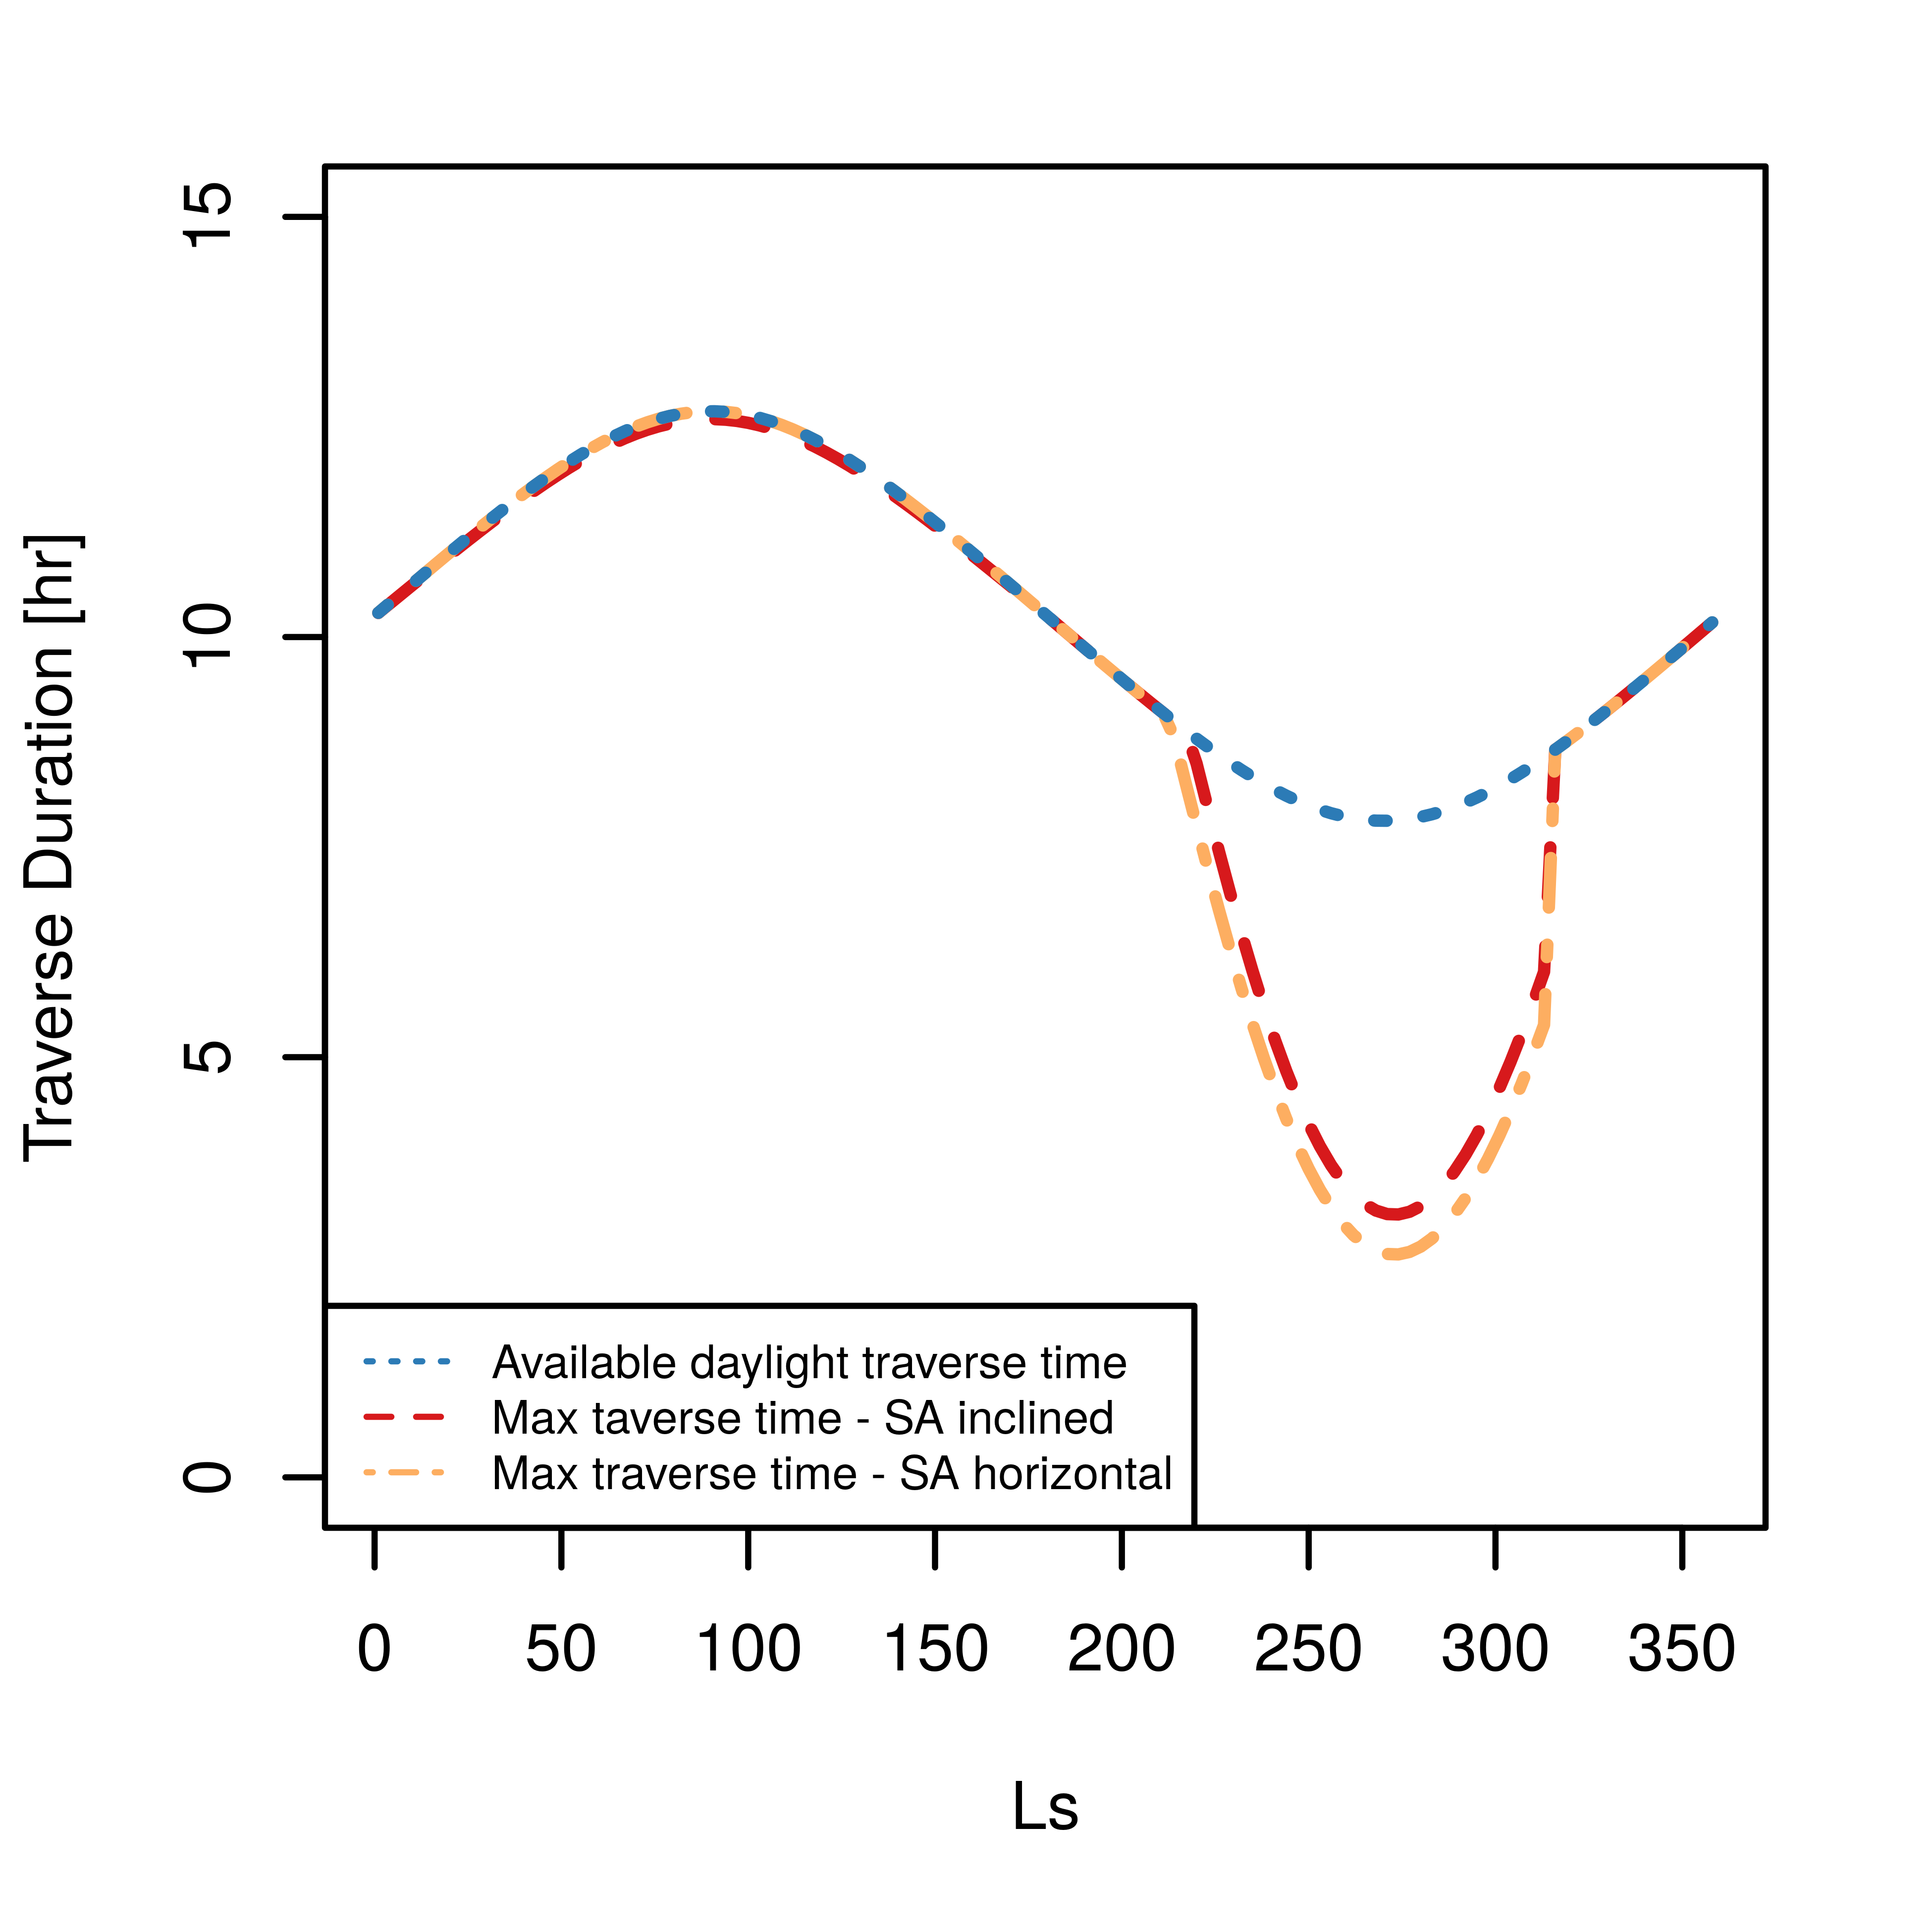
\includegraphics[height=\graphicsHeight]{sections/design/solar-array/plots/ismeniuscavus-75w-max-traverse-durations.png}
  		\subcaption{Maximum Traverse Durations}
		\label{fig:plot:sub:ismenius-cavus-max-traverse-durations}
	\end{subfigure}\\[0.8ex]
    \caption[Generated energy and maxium achievable flat terrain traverse durations at Ismenius Cavus]
            {Generated energy and maxium achievable flat terrain traverse duration at Ismenius Cavus. The same considerations were taken as in Figure \ref{fig:plot:iani-chaos-generated-energy-and-max-traverse-durations}.}
    \label{fig:plot:ismenius-cavus-generated-energy-and-max-traverse-durations}
\vspace{-2ex}
\end{figure}

\begin{figure}[h]
\captionsetup[subfigure]{justification=centering}
\vspace{-2ex}
	\centering
    %% setup sizes
    \setlength{\subfigureWidth}{0.50\textwidth}
    \setlength{\graphicsHeight}{80mm}
    %% kill hyper-link highlighting
    \hypersetup{hidelinks=true}%
    %% the figures
    \begin{subfigure}[t]{\subfigureWidth}
        \centering
        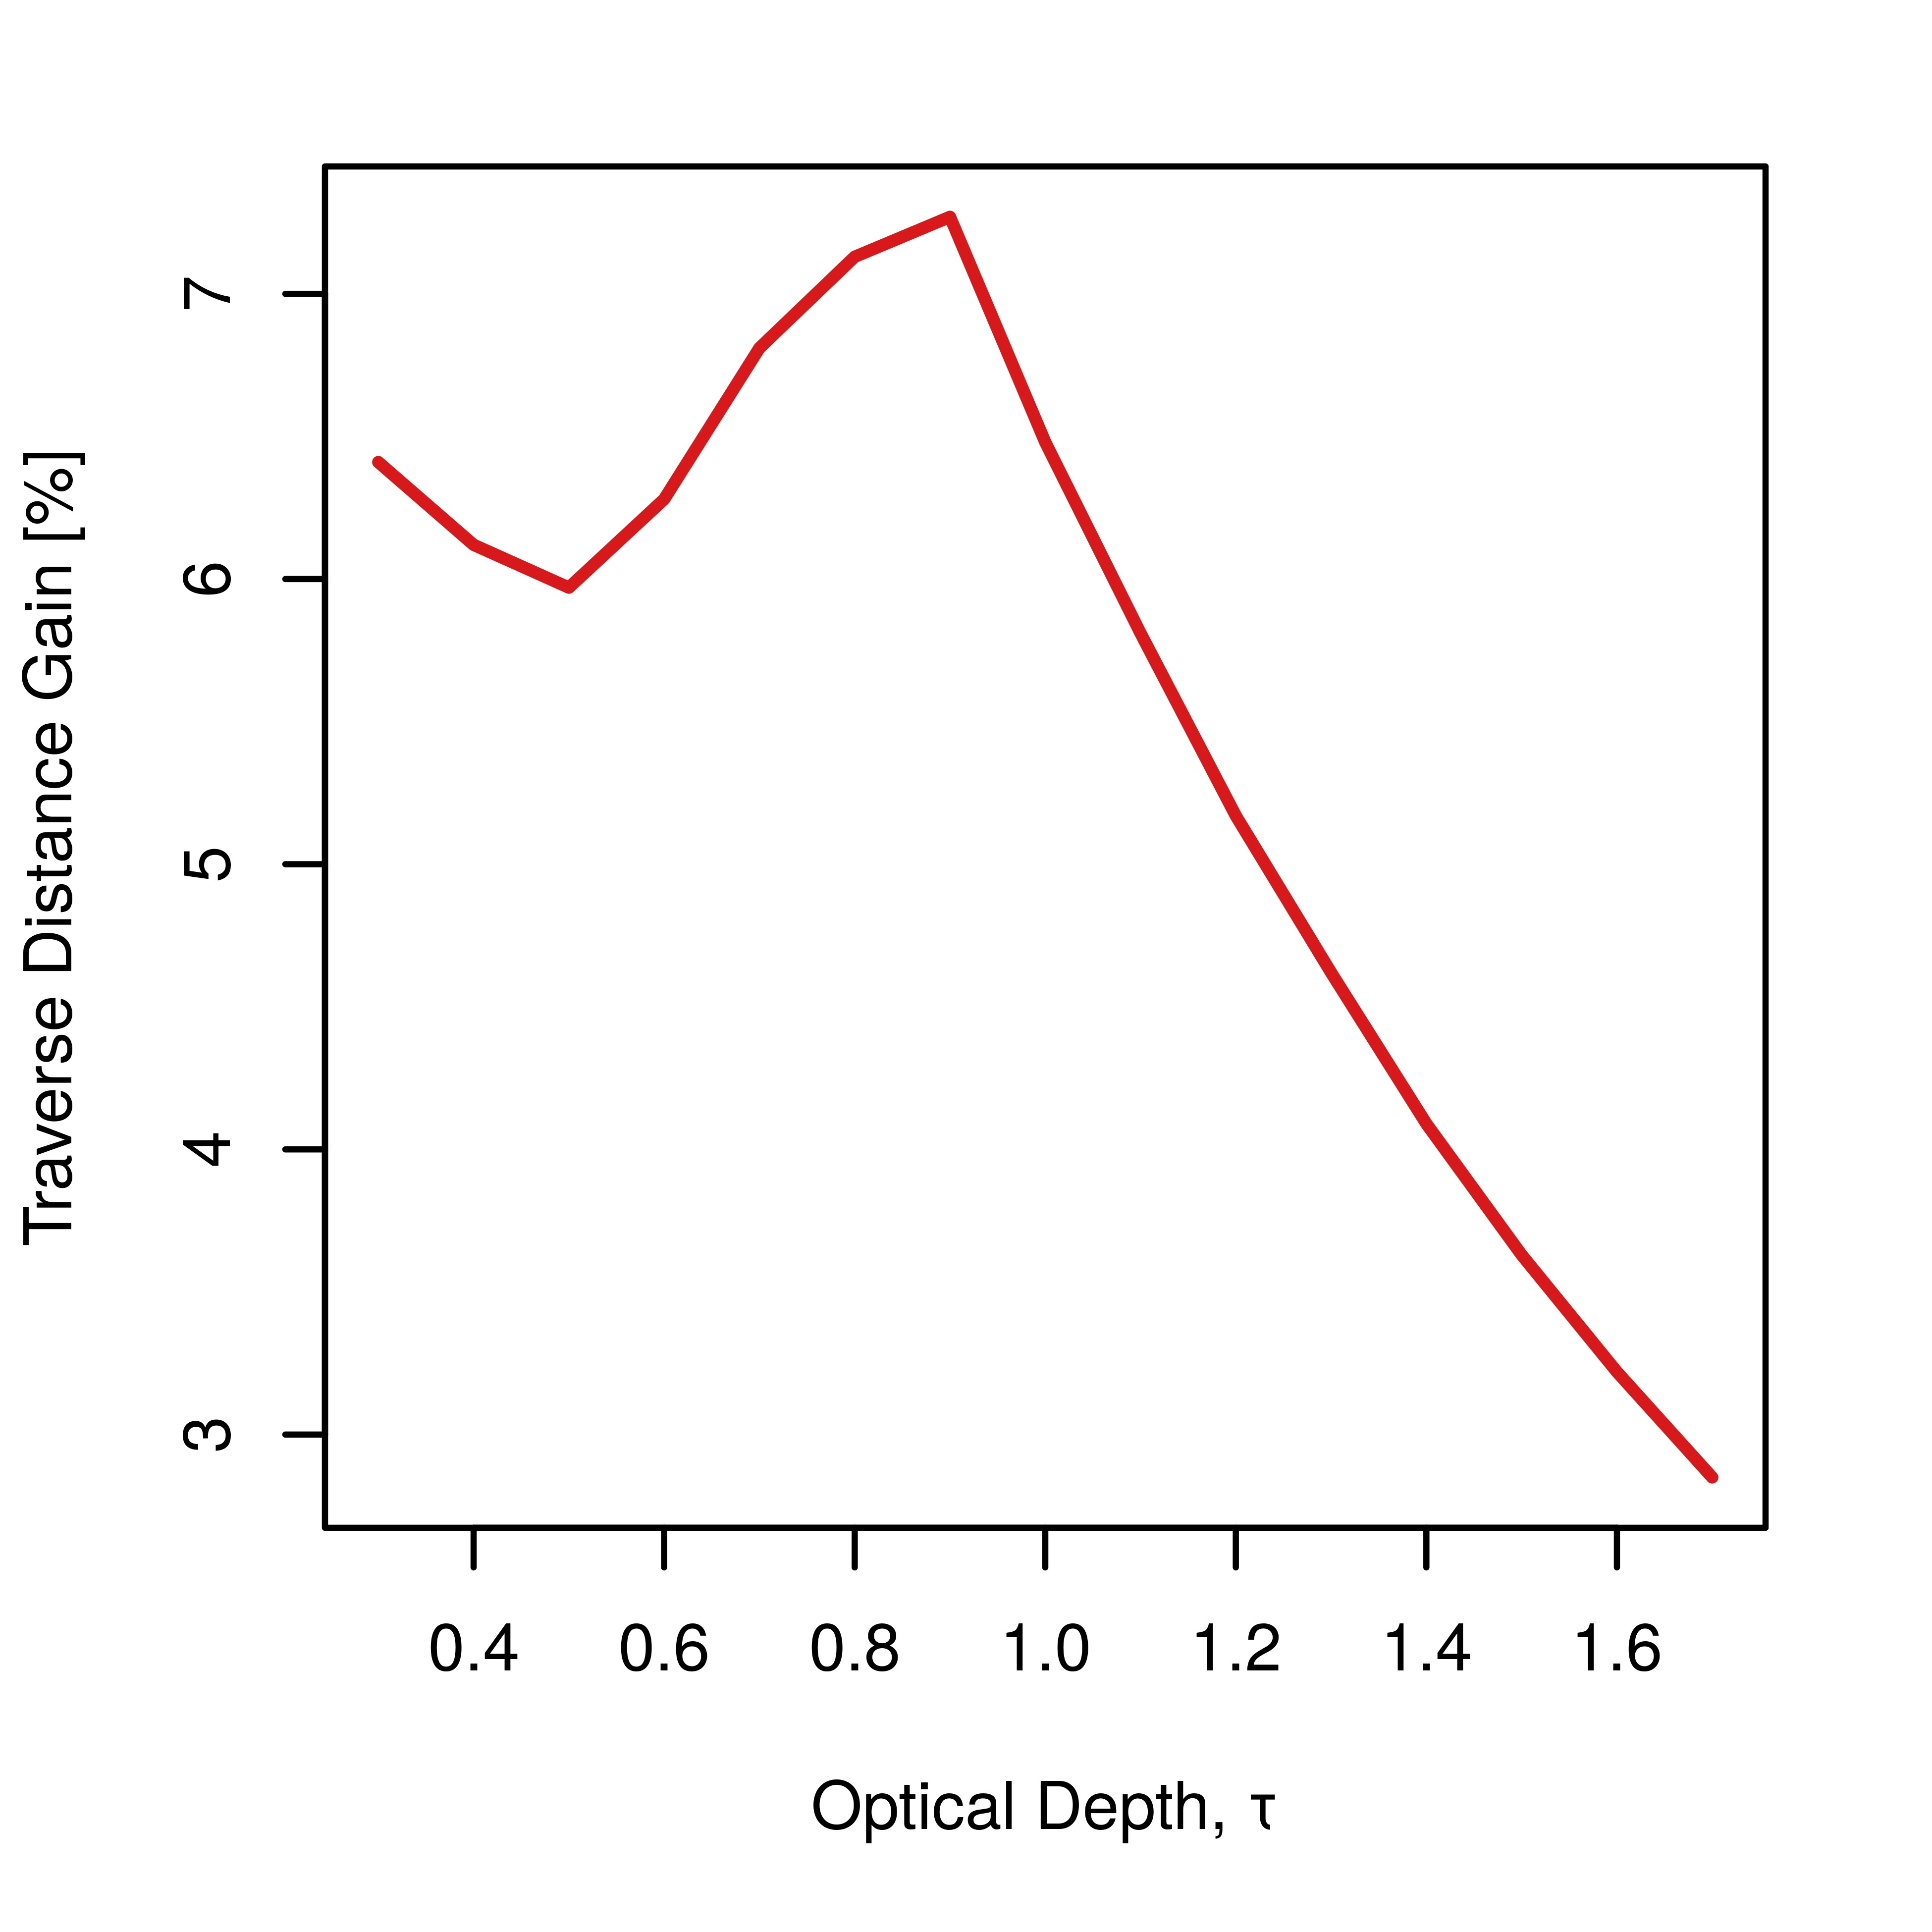
\includegraphics[height=\graphicsHeight]{sections/design/solar-array/plots/ianichaos-75w-traverse-gains-for-27m2-sa-area.png}
        \subcaption{\ac{SA} area = \SI{2.7}{\meter\squared}}
        \label{fig:plot:sub:iani-chaos-flat-traverse-gains-for-initial-sa-area}
    \end{subfigure}\hfill
    \begin{subfigure}[t]{\subfigureWidth}
        \centering
        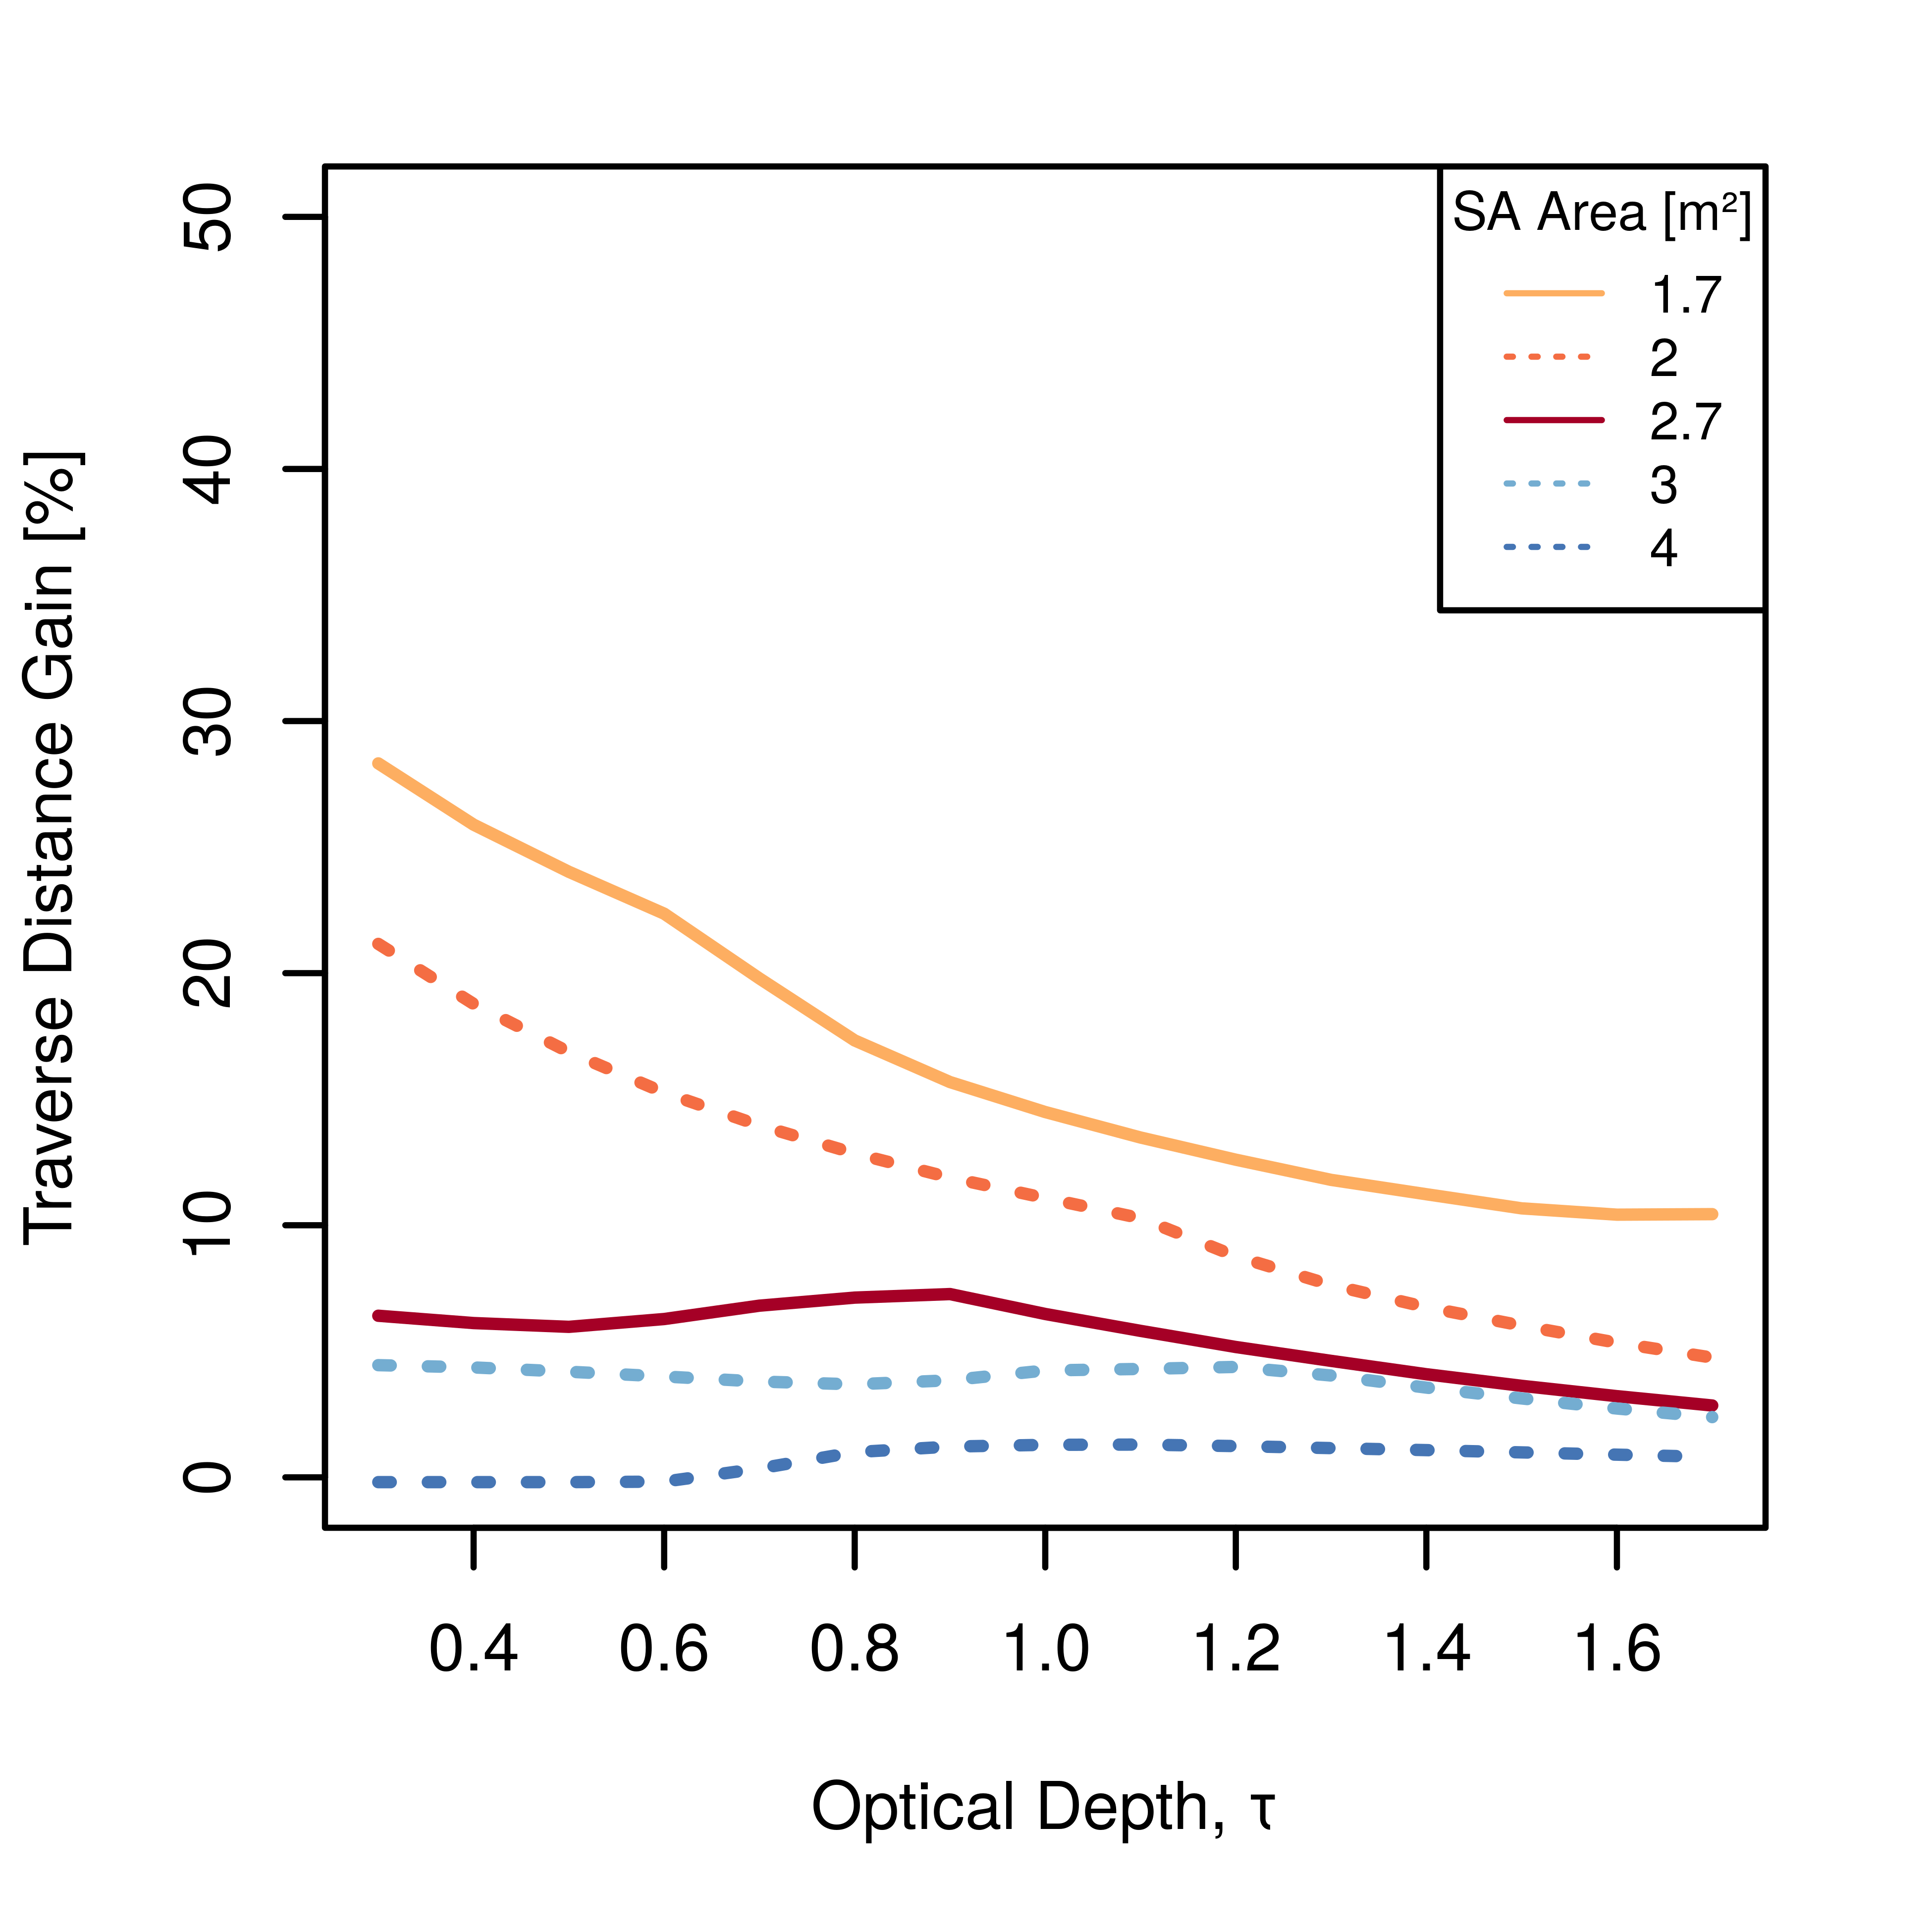
\includegraphics[height=\graphicsHeight]{sections/design/solar-array/plots/ianichaos-75w-traverse-gains-for-different-sa-areas.png}
  		\subcaption{For different \ac{SA} areas}
		\label{fig:plot:sub:iani-chaos-flat-traverse-gains-for-different-sa-area}
	\end{subfigure}\\[0.8ex]
    \caption[Flat traverse distance gains at Iani Chaos]
            {Flat traverse distance gains at Iani Chaos.}
    \label{fig:plot:iani-chaos-flat-traverse-gains}
\vspace{-2ex}
\end{figure}




\begin{figure}[h]
\captionsetup[subfigure]{justification=centering}
\vspace{-2ex}
	\centering
    %% setup sizes
    \setlength{\subfigureWidth}{0.50\textwidth}
    \setlength{\graphicsHeight}{80mm}
    %% kill hyper-link highlighting
    \hypersetup{hidelinks=true}%
    %% the figures
    \begin{subfigure}[t]{\subfigureWidth}
        \centering
        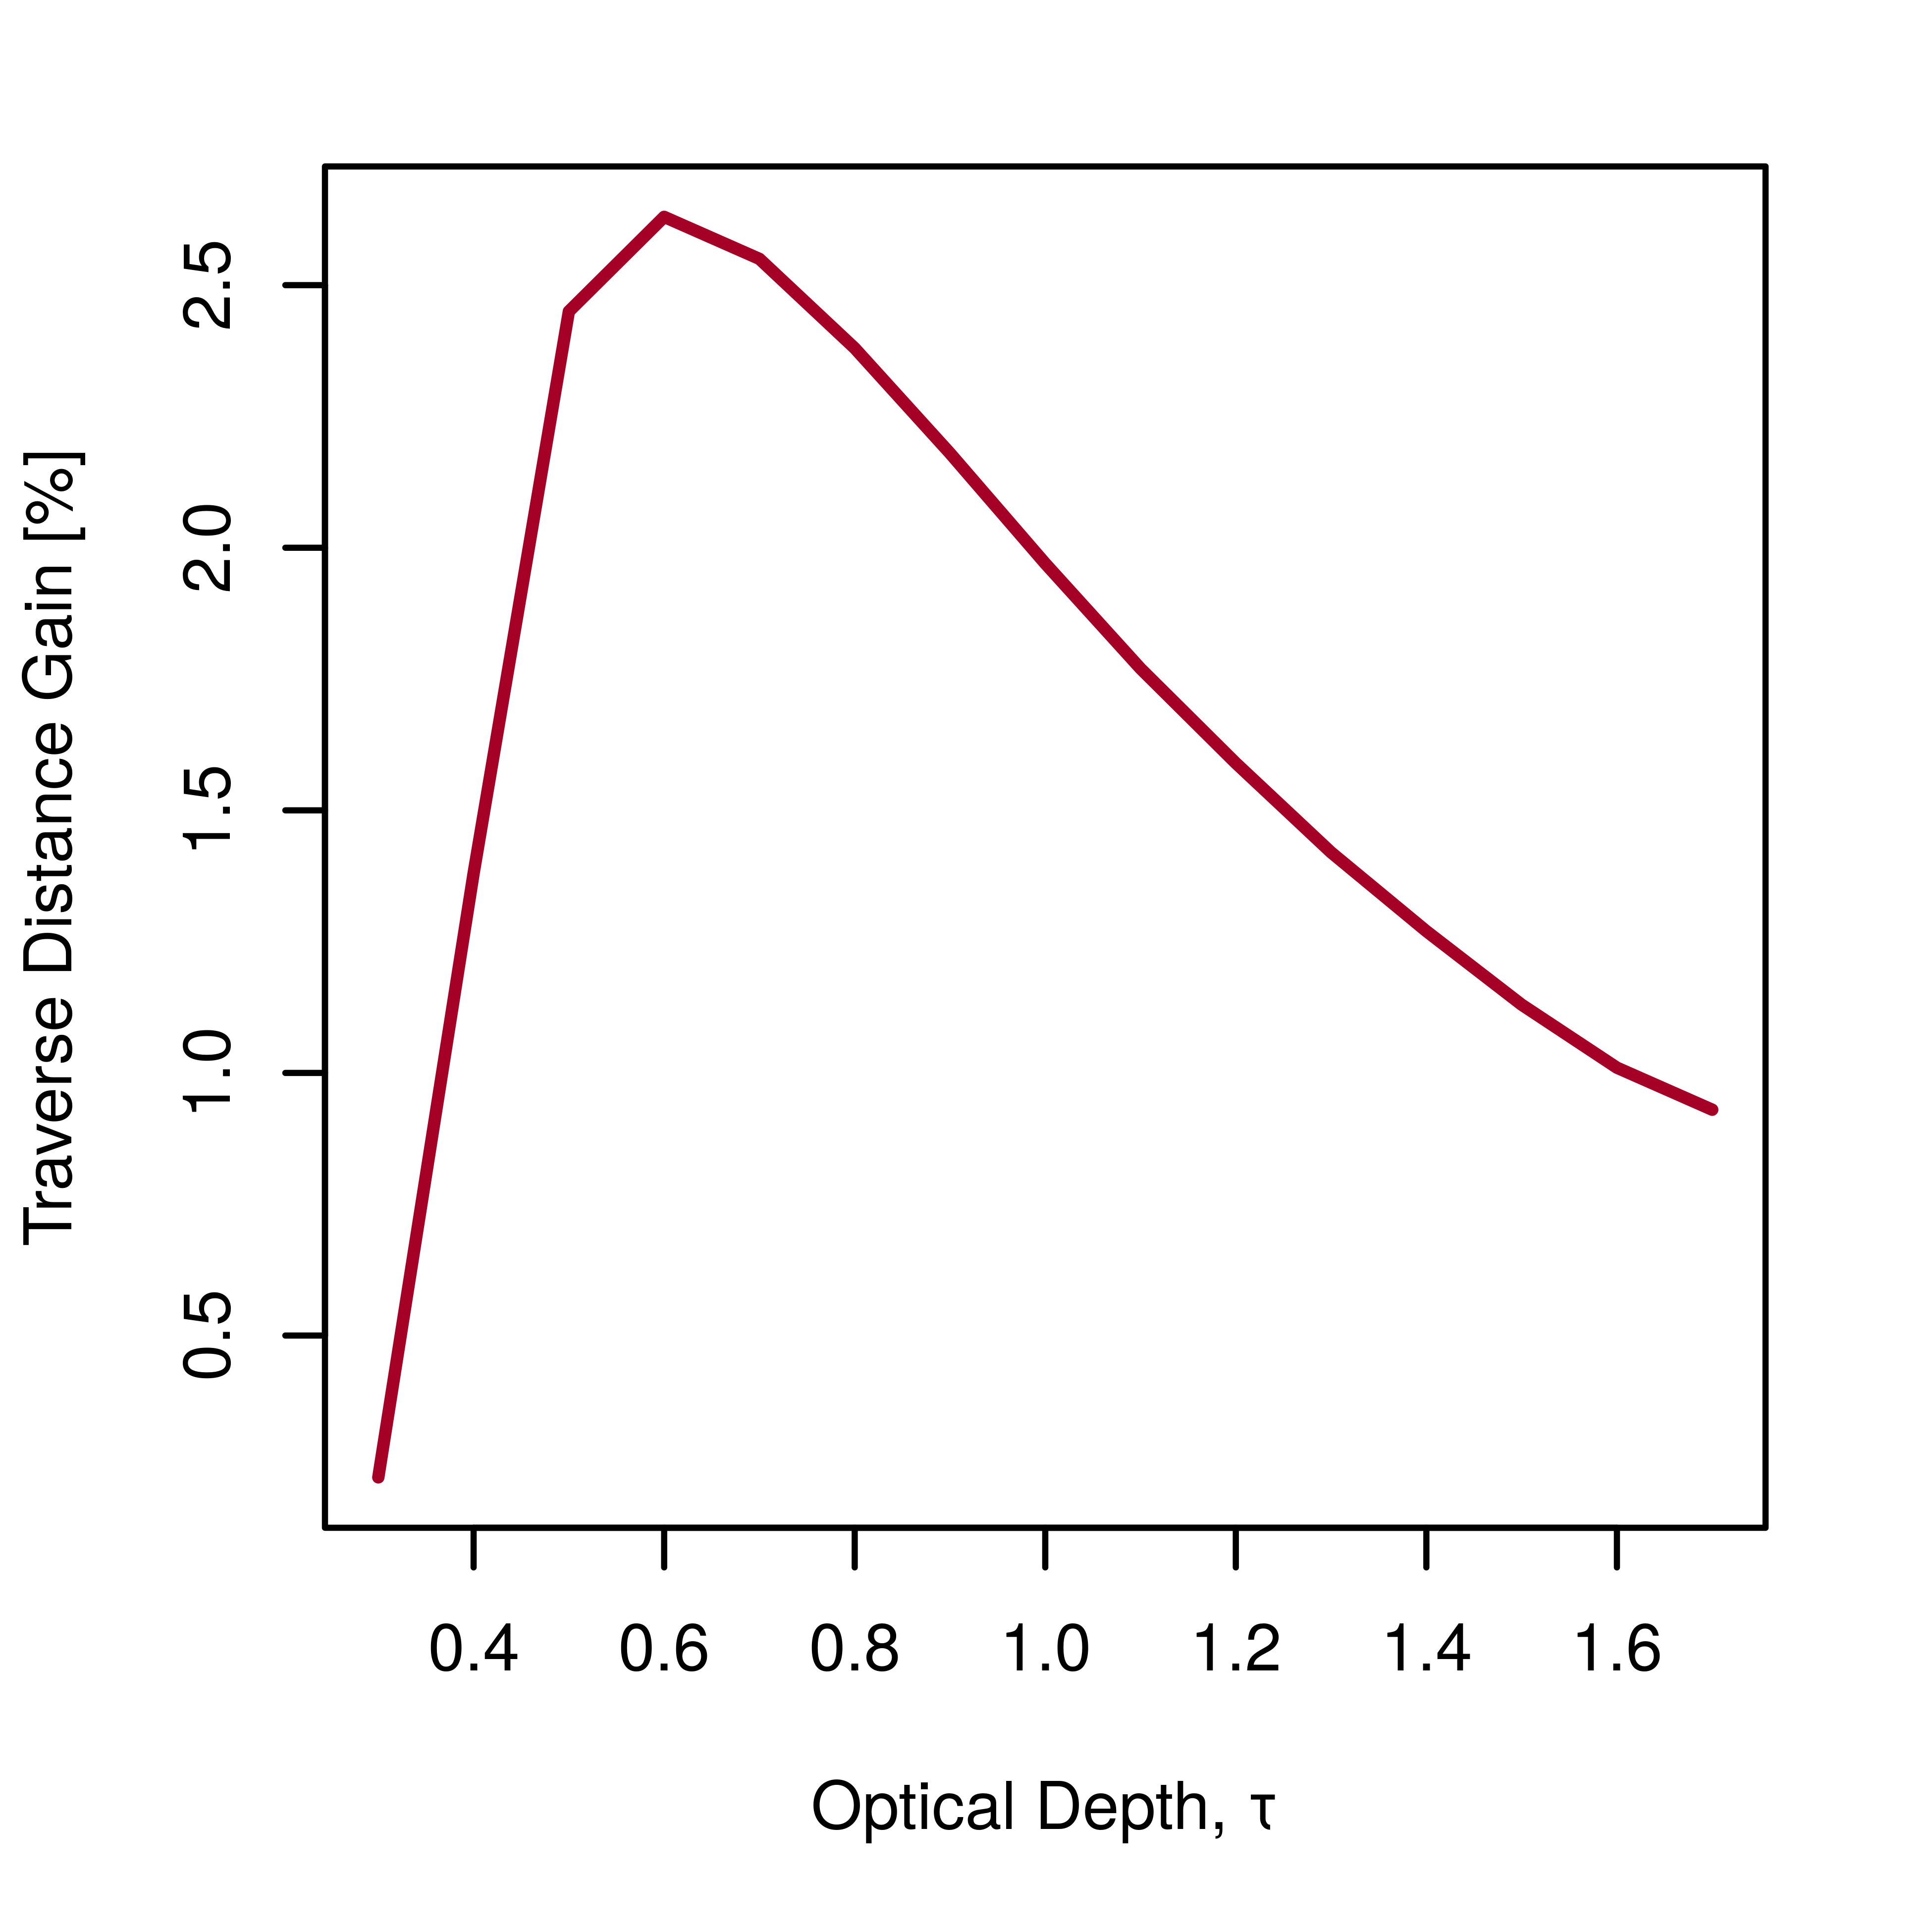
\includegraphics[height=\graphicsHeight]{sections/design/solar-array/plots/ismeniuscavus-75w-traverse-gains-for-48m2-sa-area.png}
        \subcaption{\ac{SA} area = \SI{4.8}{\meter\squared}}
        \label{fig:plot:sub:ismenius-chaos-flat-traverse-gains-for-initial-sa-area}
    \end{subfigure}\hfill
    \begin{subfigure}[t]{\subfigureWidth}
        \centering
        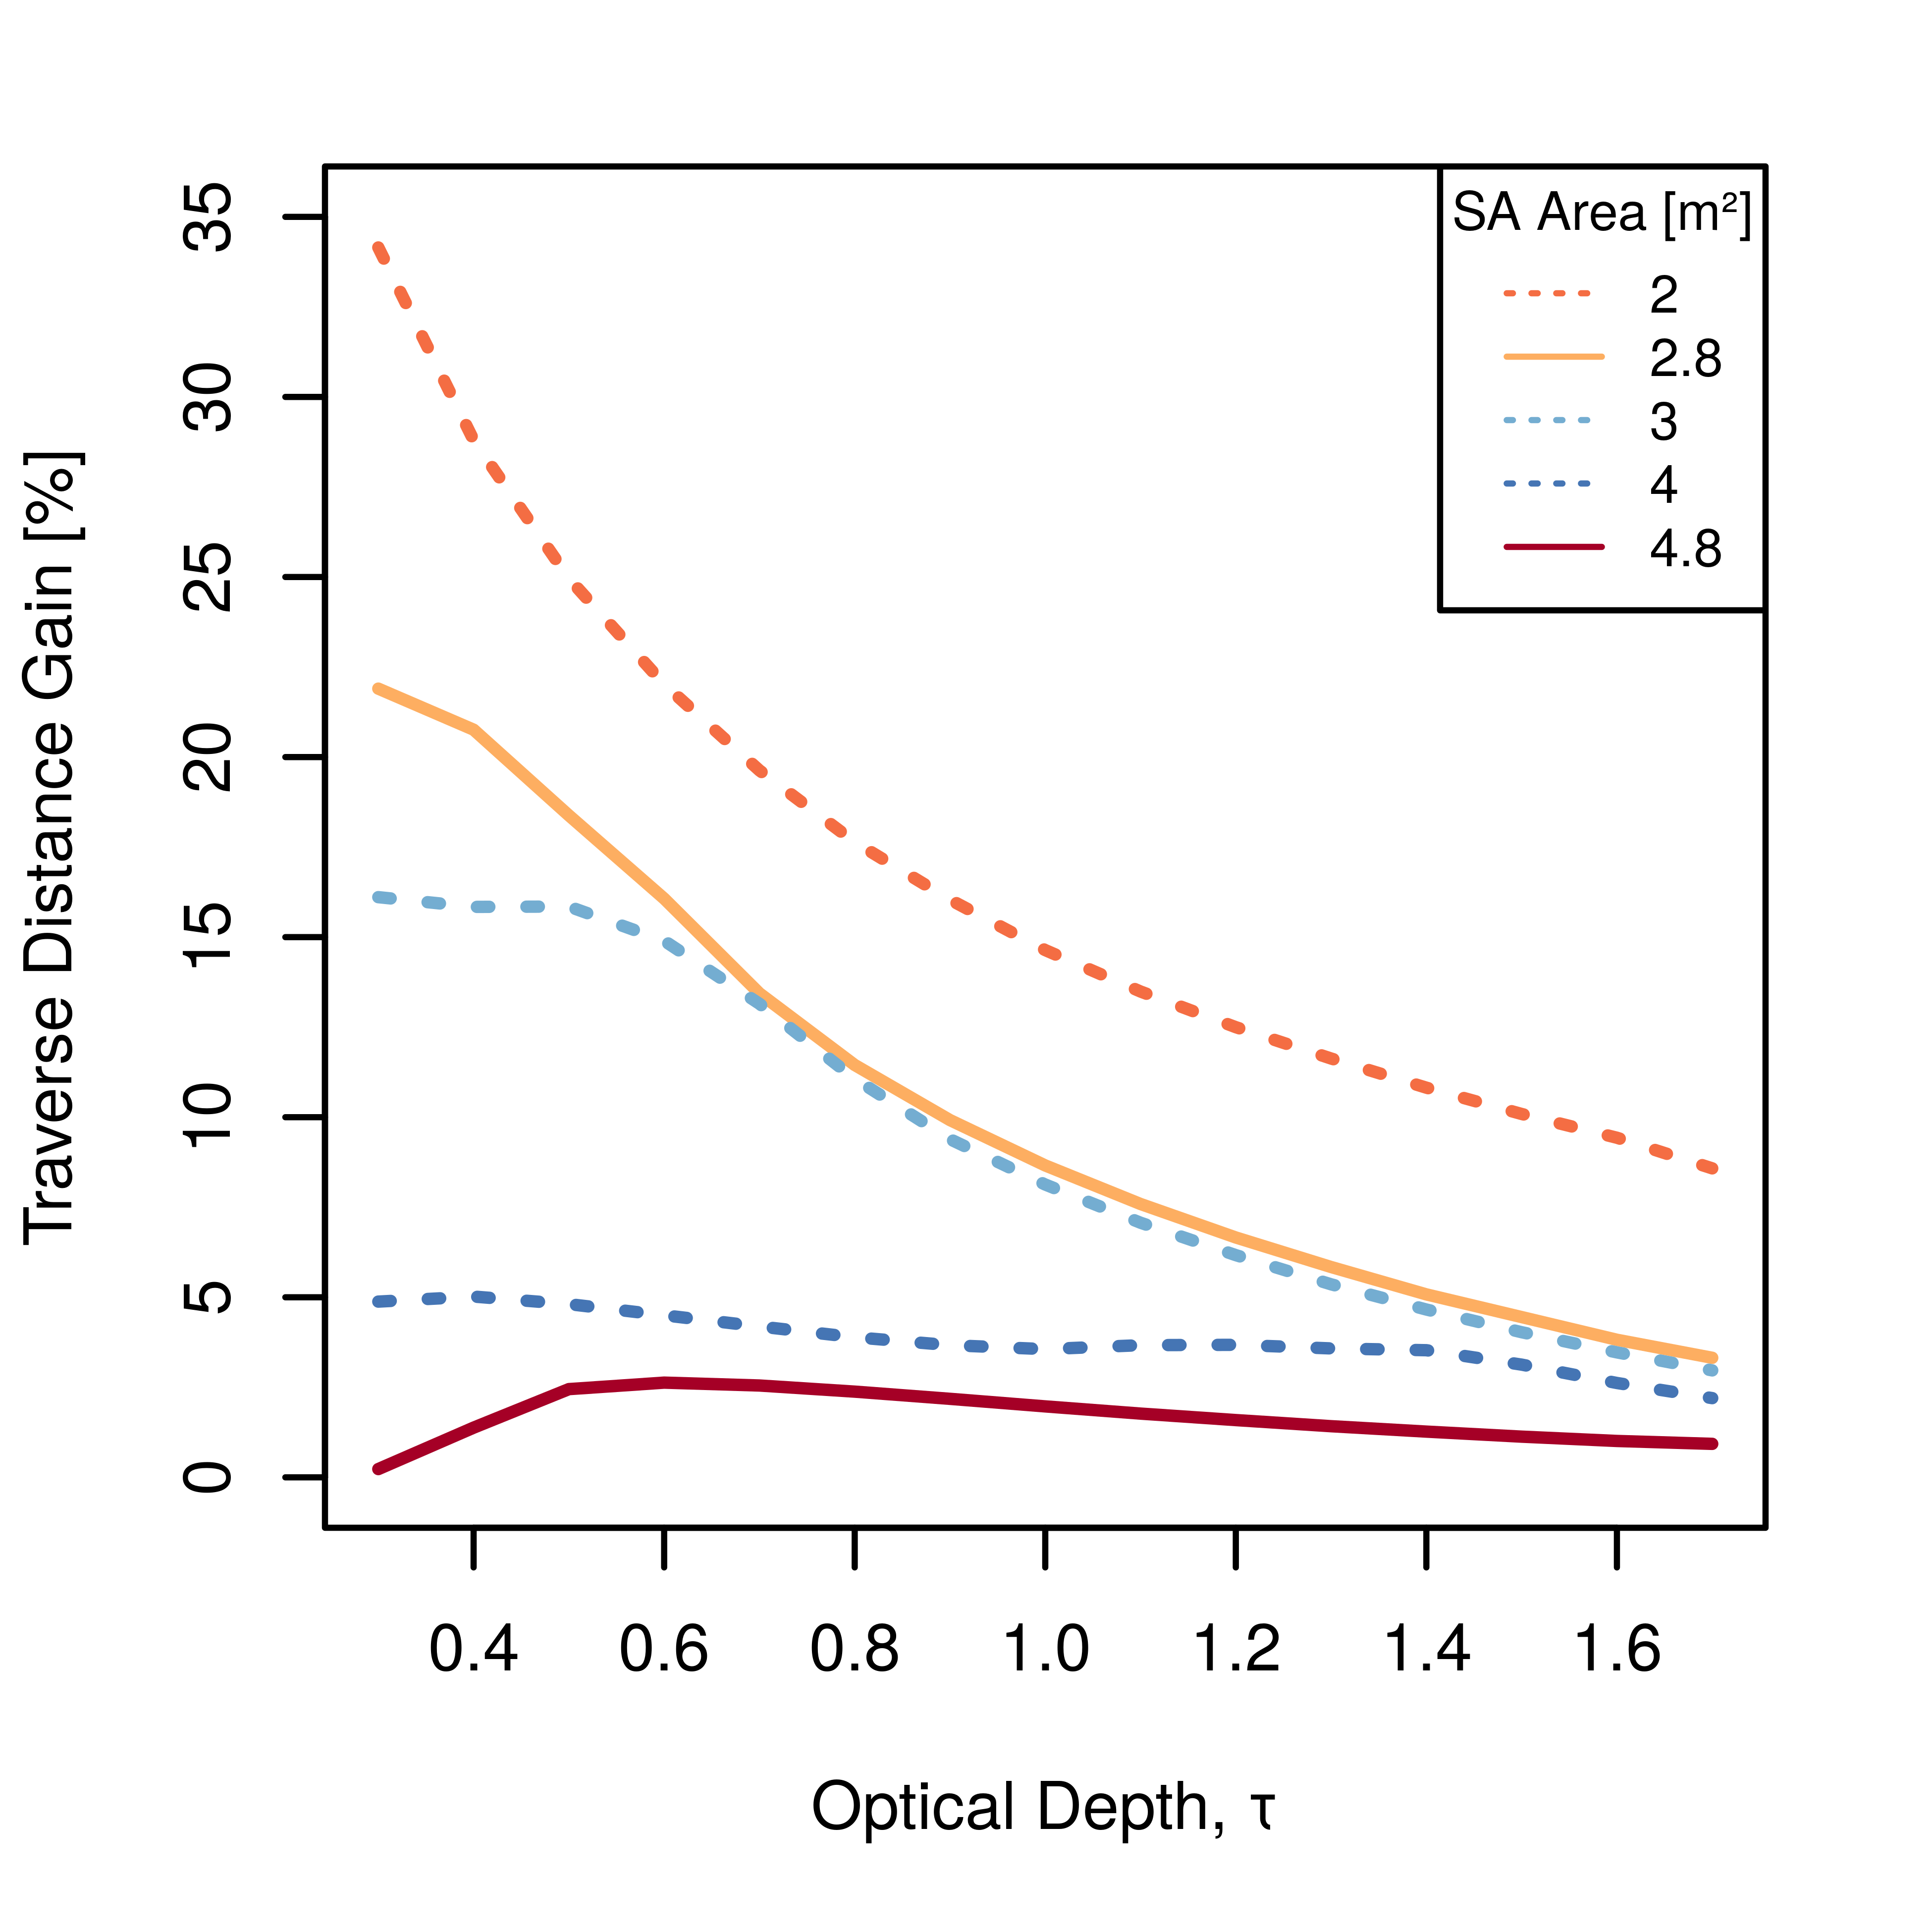
\includegraphics[height=\graphicsHeight]{sections/design/solar-array/plots/ismeniuscavus-75w-traverse-gains-for-different-sa-areas.png}
  		\subcaption{For different \ac{SA} areas}
		\label{fig:plot:sub:ismenius-chaos-flat-traverse-gains-for-different-sa-area}
	\end{subfigure}\\[0.8ex]
    \caption[Flat traverse distance gains at Ismnenius Chaos]
            {Flat traverse distance gains at Ismnenius Chaos.}
    \label{fig:plot:ismenius-chaos-flat-traverse-gains}
\vspace{-2ex}
\end{figure}


\todo[inline]{\textbf{TODO:} Size SA with hibernation power budget. Reduce Hibernation mode power draw.}

%\label{itm:req:total_distance_flat_terrain}

\clearpage
\subsubsection{Battery}
\todo[inline]{\textbf{TODO:} Battery size based on energy required to keep the rover Warm through the night. Check if the calculated size satisfies the hibernation requirement. If not, resize.}

\subsection{Baseline Design}
\todo[inline]{\textbf{TODO:} Refer to design drivers and present solution.}

\subsection{Mechanisms}
\todo[inline]{\textbf{TODO:} Short introduction.}

\subsubsection{Deployment}
\todo[inline]{\textbf{TODO:} 1. Sequence and 2. Cantilever beam analysis at every deployment step.}

\subsubsection{HDRMs}
\todo[inline]{\textbf{TODO:} Calculate for Force acting on the \ac{HDRM}.}

\subsection{Summary}
\todo[inline]{\textbf{TODO:} Write section summary.}
